

\chapter{Noise Reduction through De-Whitening Filter}

\section{Concept of De-Whitening Filter}
Considering a situation in which the Photon Calibrator received white, i.e.~frequency independent, excitation signal noise, it will generate $1/f^2$ displacement noise on End-Test-Mirror because the force-to-displacement transfer function contains a $1/f^2$ feature. If we put an analog filter that has frequency response proportional to $f^2$ between the excitation signal and the PCal excitation input port, we may create colored, $f^2$, laser intensity noise from white electrical noise of the excitation signal. Then, such colored noise will be whitened by the $1/f^2$ force-to-displacement transfer function, becoming white displacement noise. We call the $f^2$ analog filter \emph{De-Whitening filter}.


Practically, we use a single zero-pole analog filter with transfer function shown in Fig.(\ref{fig:DEWtf_design}) as our De-Whitening filter. 

\begin{figure}[hbt!]
\centering
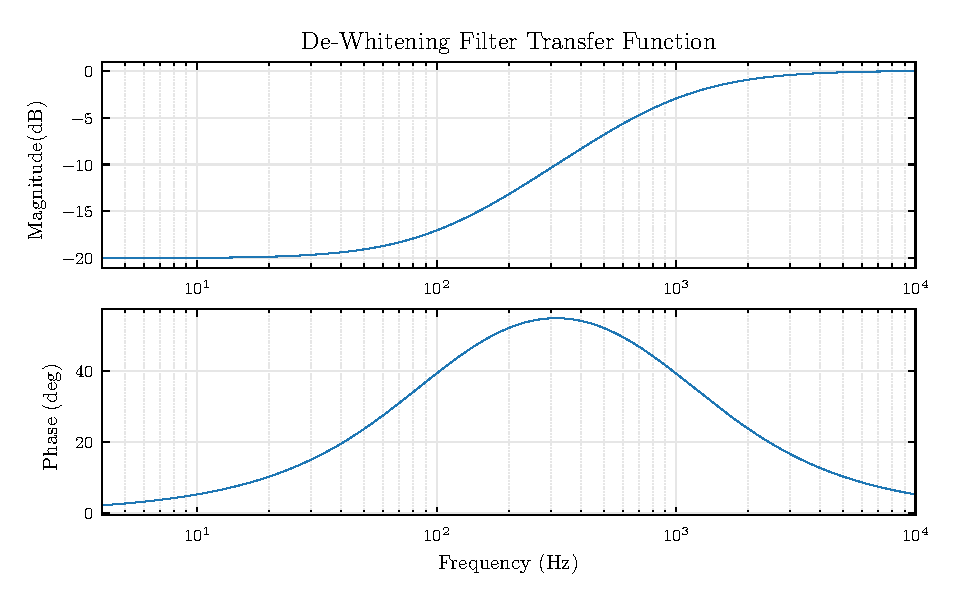
\includegraphics[width=1\textwidth]{figure/DEWtf_design}
\caption[De-Whitening filter transfer function]{De-Whitening filter transfer function. This is the designed transfer function of De-Whitening filter. It has a pole at 1kHz and a zero at 100Hz. }
\label{fig:DEWtf_design}
\index{figures}
\end{figure}





\section{Circuit Design}
The main circuit design is described in Fig.~\ref{fig:dewcircuit}. It converts a differential input signal into a single-ended one by an instrumentation amplifier. Then, the signal will pass through the De-Whitening stage, which attenuates the low-frequency signal while keeping the gain of the high-frequency signal unchanged. After that, we convert the filtered single-ended output to differential output, and send it to a downstream device.


The frequency dependent attenuation in the De-Whitening stage is realized by a single zero-pole analog filter. The pole and zero frequencies are determined by resistors and capacitors between A and B in Fig.~\ref{fig:dewcircuit}. In order to reduce filter shape uncertainty caused by pole-zero frequency drifting, we use 0.01$\mu$F Mica capacitor (CD30FD103FO3F made by Cornell Dubilier Electronics), whose capacitance tolerance is within 1\% and capacitance drift is within $\pm(0.05\% +0.1 pF)$.

The transfer function of this circuit is
%\begin{equation}
%    \frac{(1+ i \omega R_b C)}{(1+\frac{R_b}{R_a}) + (i \omega R_b C )}
%\end{equation}

\begin{equation}
\label{eq:dewtf}
    \mathrm{DewTF} = \underbrace{\frac{Z_A}{Z_A+Z_B}}_{\text{pole-zero stage}} \times \underbrace{2}_{\text{Single to Differential}}
\end{equation}
where
\begin{align}
    A//B &\equiv \frac{1}{\frac{1}{A}+\frac{1}{B}} \\
    Z_B &= ( R_3 + \frac{1}{i \omega C_2} )~ //~ R_b \\
    Z_A &= ( R_4 + \frac{1}{i \omega C_1} )~ //~ R_a
\end{align}
When $R_3=R_4=a$, $C1=C2=C$, Eq.~(\ref{eq:dewtf}) will reduce to 
\begin{equation}
%\label{eq:dewtf}
    \mathrm{DewTF} = 2 \left( \frac{1+i \omega C (a+ R_b)}{1+\frac{R_b}{R_a} + i \omega C (2 R_b + a(1+\frac{R_b}{R_a}))} \right)
\end{equation}
Practically, we chose $a=100\Omega << R_a =8.34(88)\mathrm{k}\Omega < R_b =159.(3)\mathrm{k}\Omega $ due the the availability of resistors in the market. Then, the DC gain is 
\begin{equation}
%\label{eq:dewtf}
    \mathrm{DewTF}\ \rvert_{\omega=0} = \frac{2}{1+\frac{R_b}{R_a}} = 0.0996
\end{equation}
It is about a factor of ten suppression of low-frequency signals while gains of high-frequency signals are kept unity.
The pole and zero frequencies of such circuit are
\begin{align}
%\label{eq:dewzp}
    \mathrm{Zero} &= \frac{1}{2 \pi C (a+R_a)} = 99.8 \mathrm{Hz} \\
    \mathrm{Pole} &= \frac{1}{2 \pi C (a+2\frac{R_a R_b}{R_a+R_b})} = 996.8 \mathrm{Hz}
\end{align}
% An overall transfer function simulated with LTspice is shown in Fig. XX 

%\begin{figure}[hbt!]
%\centering
\begin{sidewaysfigure}
%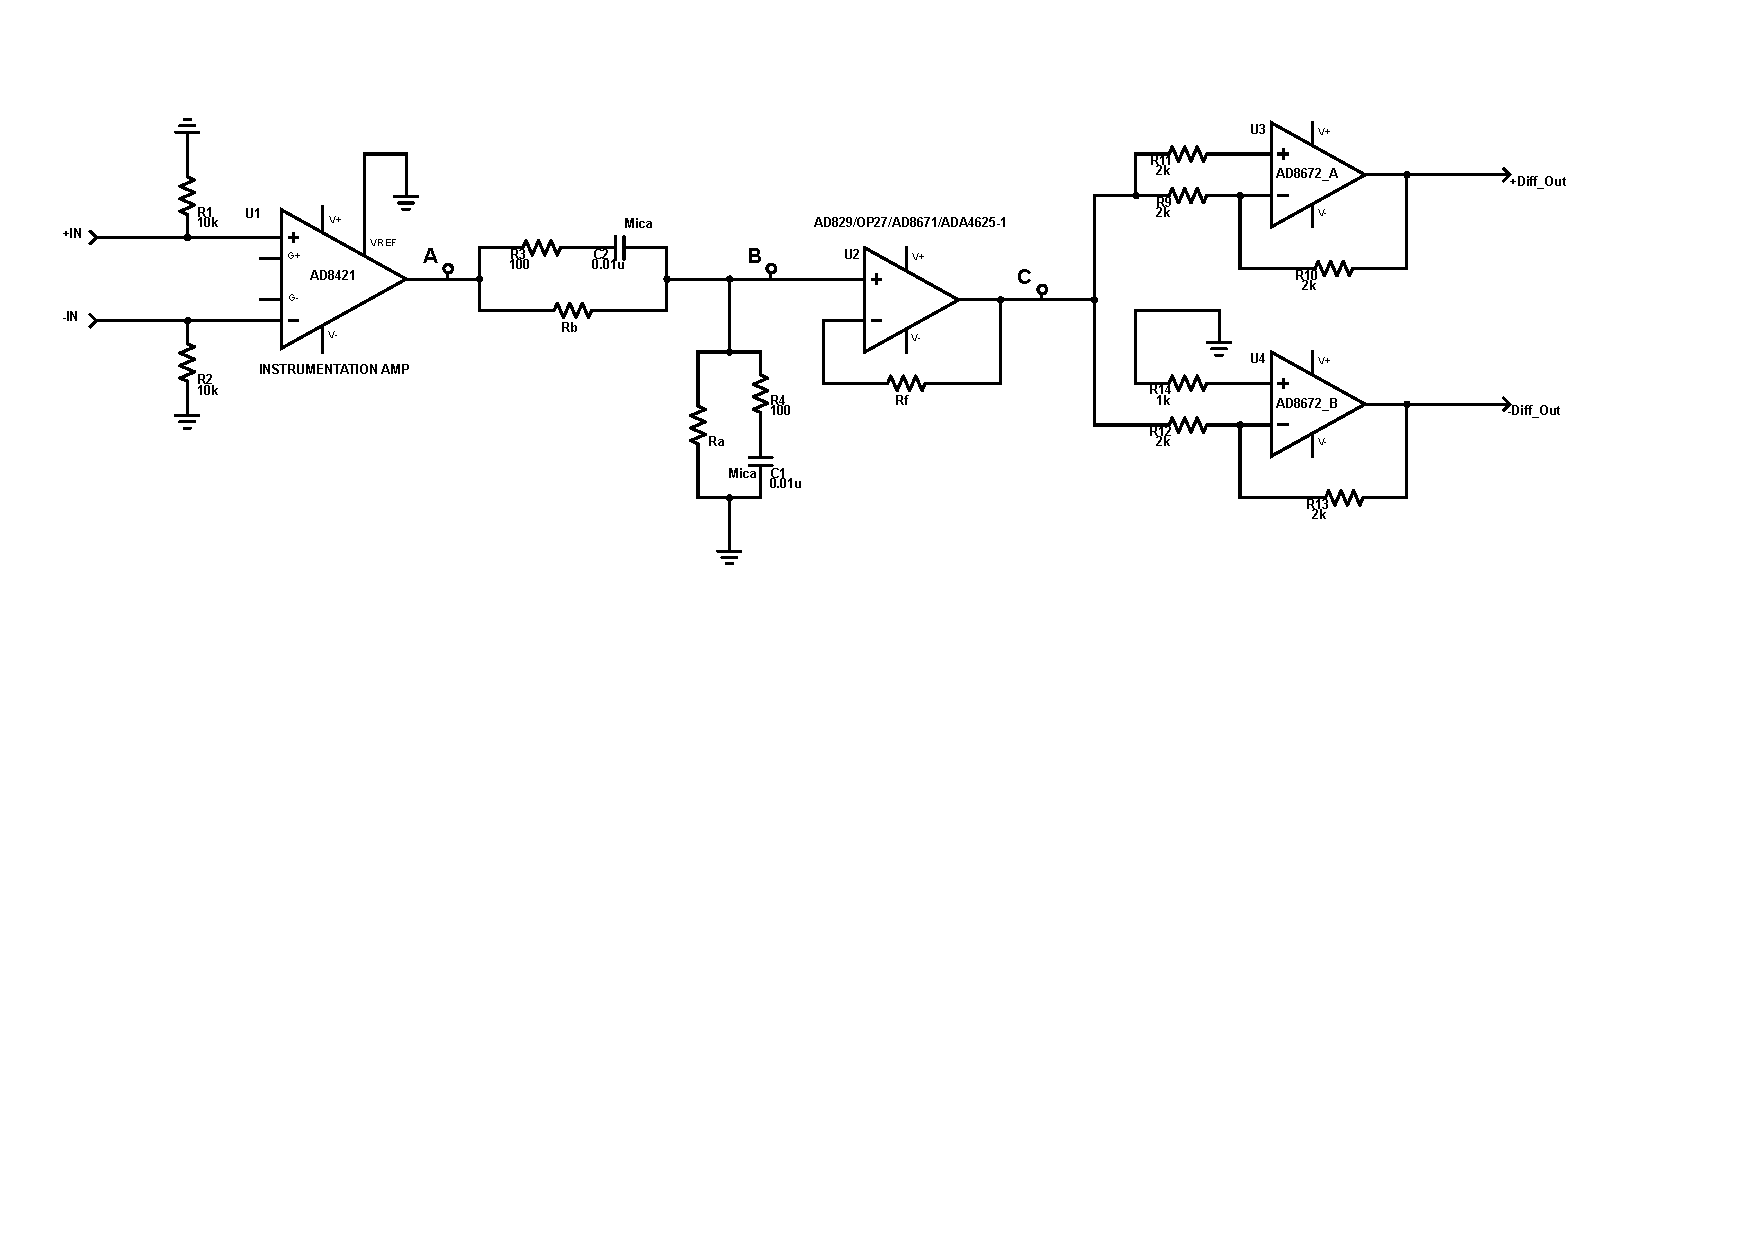
\includegraphics[angle=90, width=0.48\textwidth]{figure/DEWcircuit.pdf}
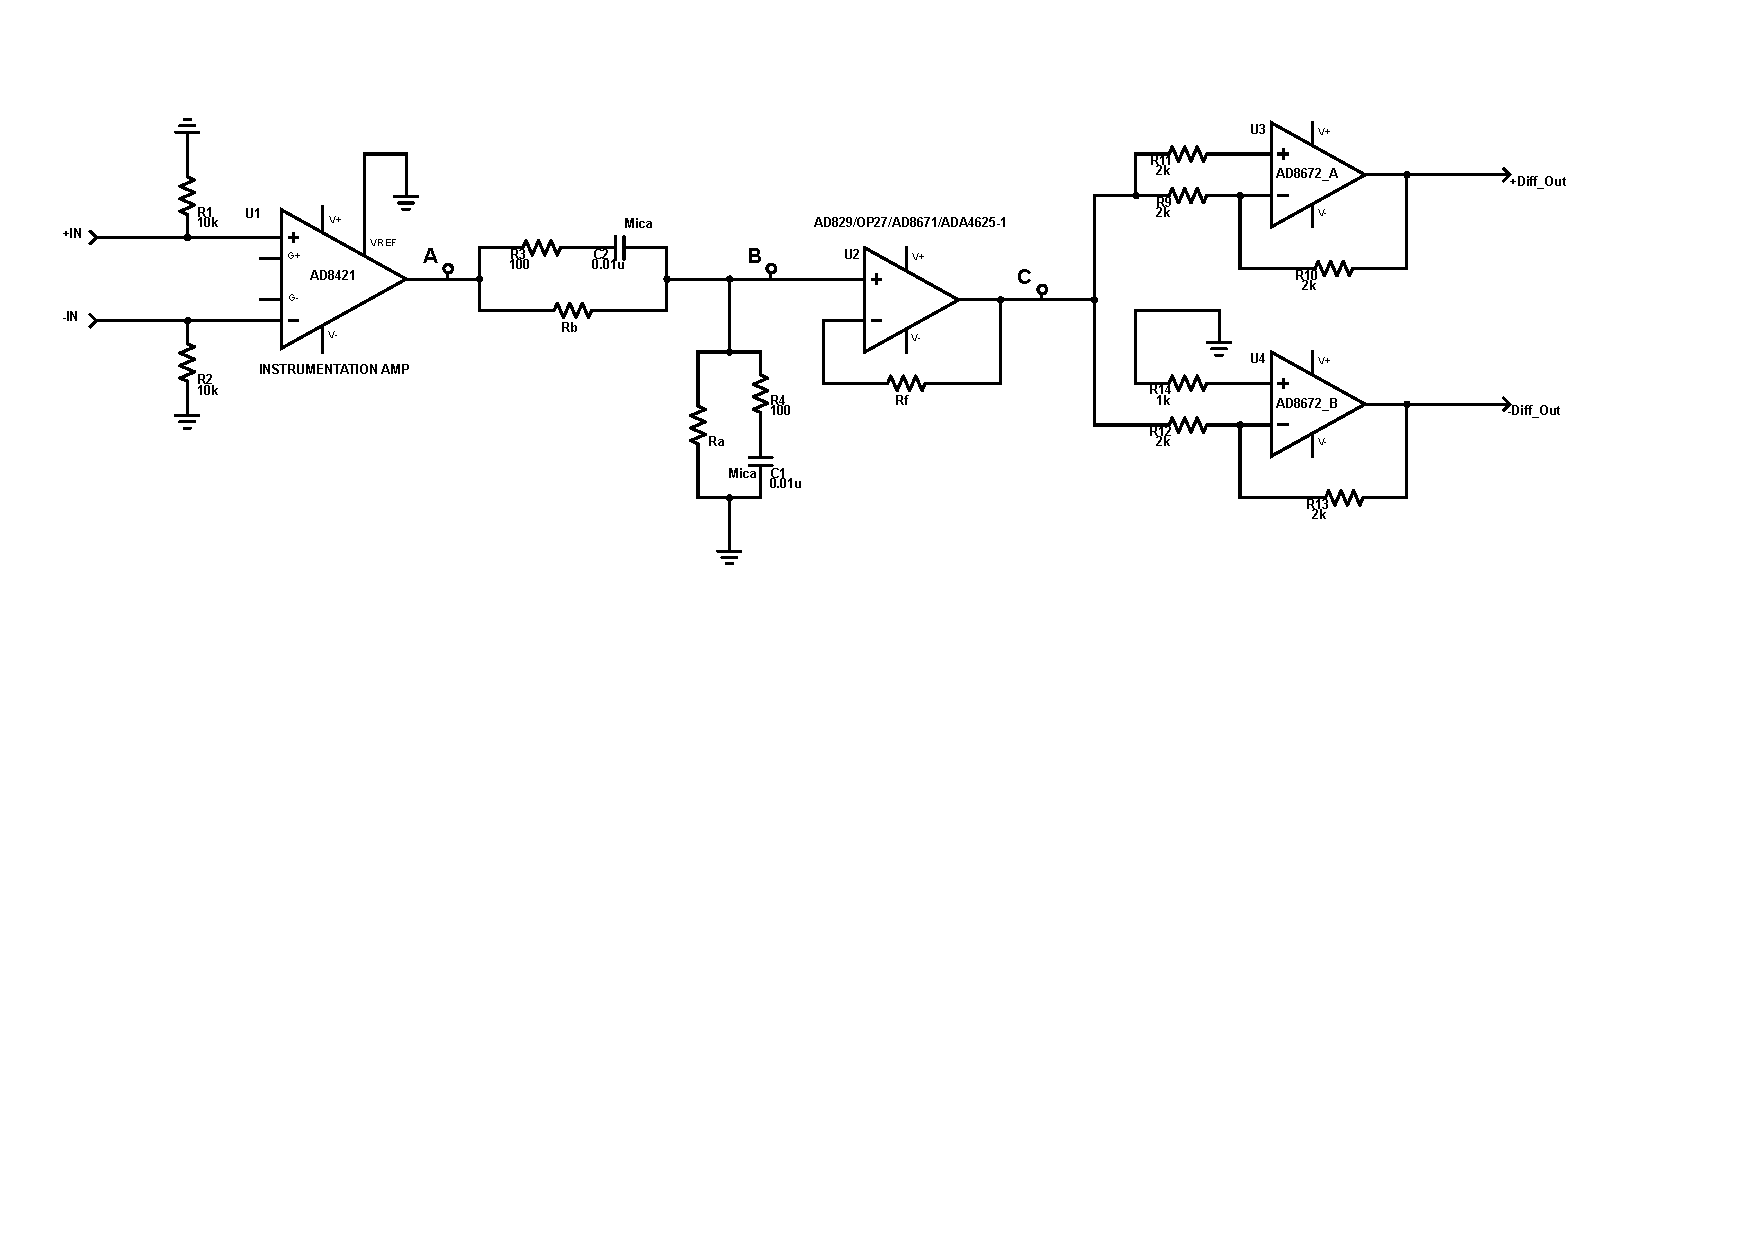
\includegraphics[width=1\textwidth]{figure/DEWcircuit.pdf}
\caption[De-Whitening filter circuit]{De-Whitening filter circuit. There are three points labeled as A, B, and C in the diagram. Before A, a differential input signal provided by Digital System will be converted into a single-ended signal by an instrumentation amplifier AD8421. After that, a passive pole-zero stage between A and B defines the dominate transfer function of the De-Whitening filter. Then we put a voltage follower between B and C as a buffer to keep passive filter response. Finally, we convert the signal back to a differential output to match the downstream device input. }\label{fig:dewcircuit}
\index{figures}
\end{sidewaysfigure}
%\end{figure}


\begin{figure}[hbt!]
\centering
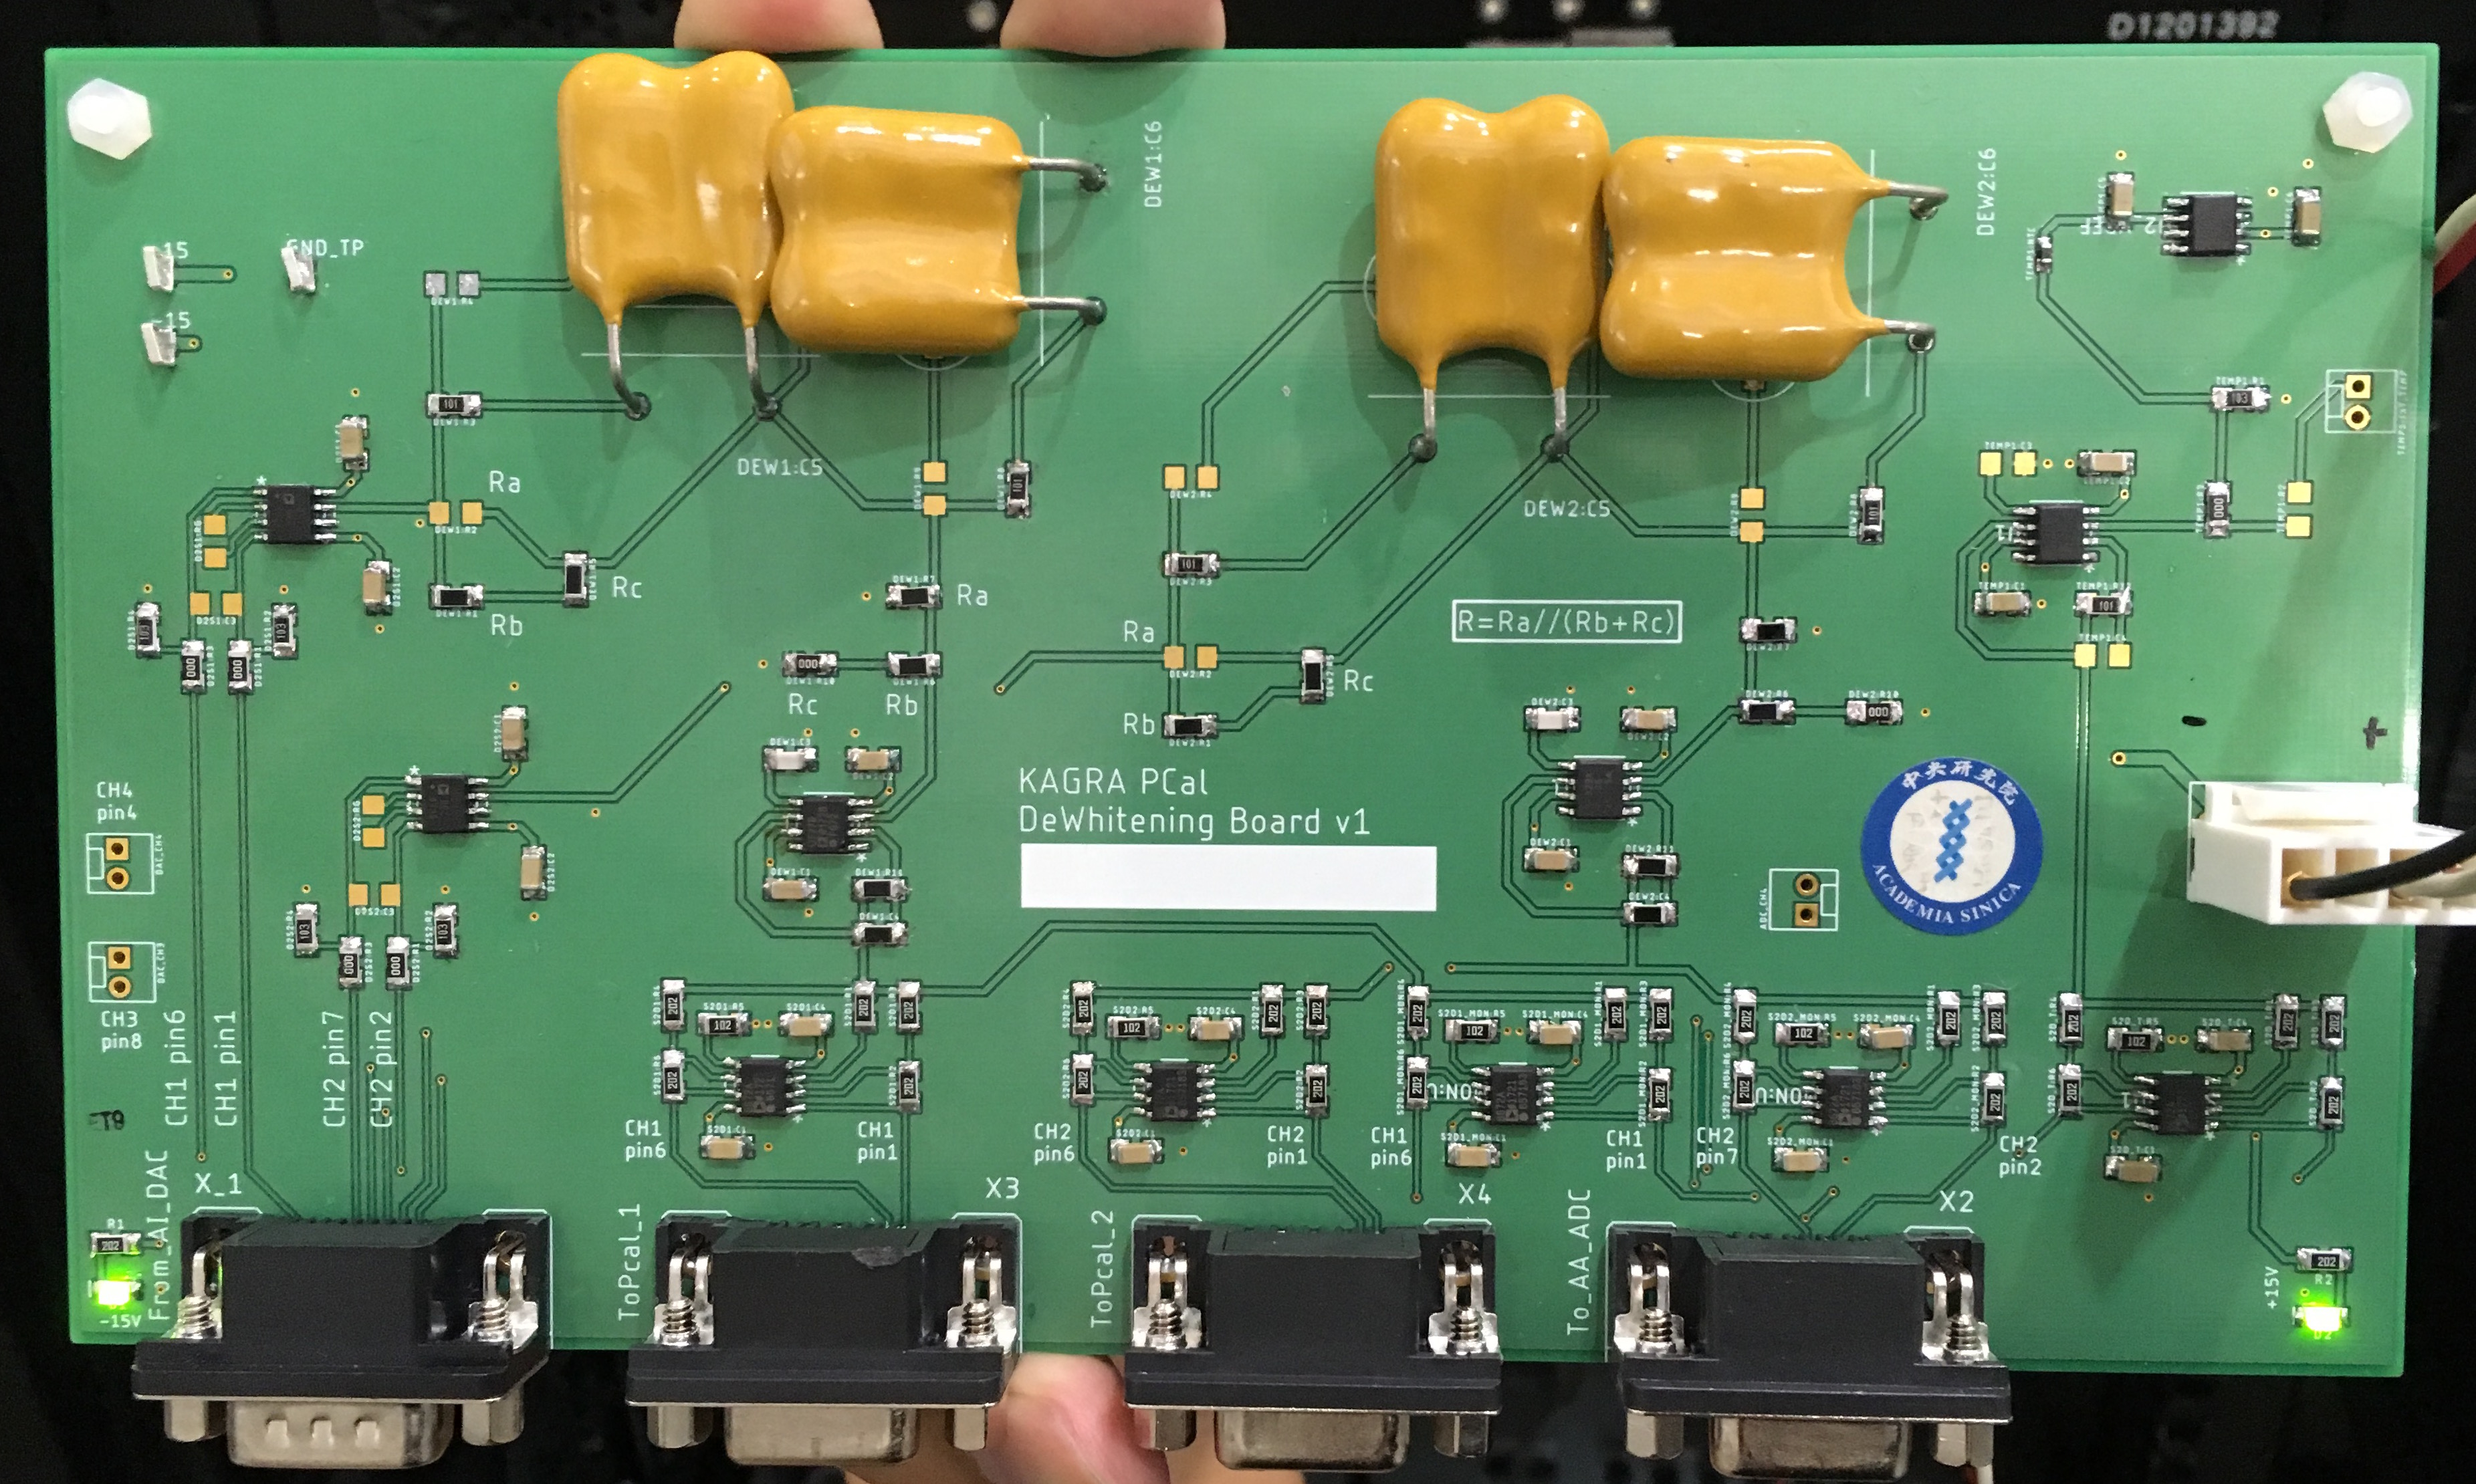
\includegraphics[width=1\textwidth]{figure/dewPhoto.jpg}
\caption[De-Whitening filter board]{De-Whitening filter board. It's a 1.6mm FR-4 printed circuit board manufactured by SPEEDY Circuits Co., Ltd. The layout of this board is done with EAGLE, an EDA software. Four large yellow capacitors are Mica capacitors for the pole-zero stage. At KAGRA site, we installed it into a 1U chassis powered by a DC power supply with a LM2941/LM2991 voltage regulation circuit designed by LIGO.}
\label{fig:board}
\index{figures}
\end{figure}



\pagebreak
\section{Fidelity of Injection Signals}
%\subsection{Transfer Function of De-Whitening Filter}
The fidelity of injected signals is the fundamental requirement of hardware injection test. One can estimate the distortion of the injected waveforms by measuring the transfer function between an excitation port in the software and the PCal laser intensity. After measuring such transfer function, we can create an inverse De-Whitening digital filter in software side to compensate for our analog De-Whitening filter. The combination allows as to suppress low-frequency noise from DAC while the transfer function for signal is kept unity.


\begin{figure}[bt!]
\centering
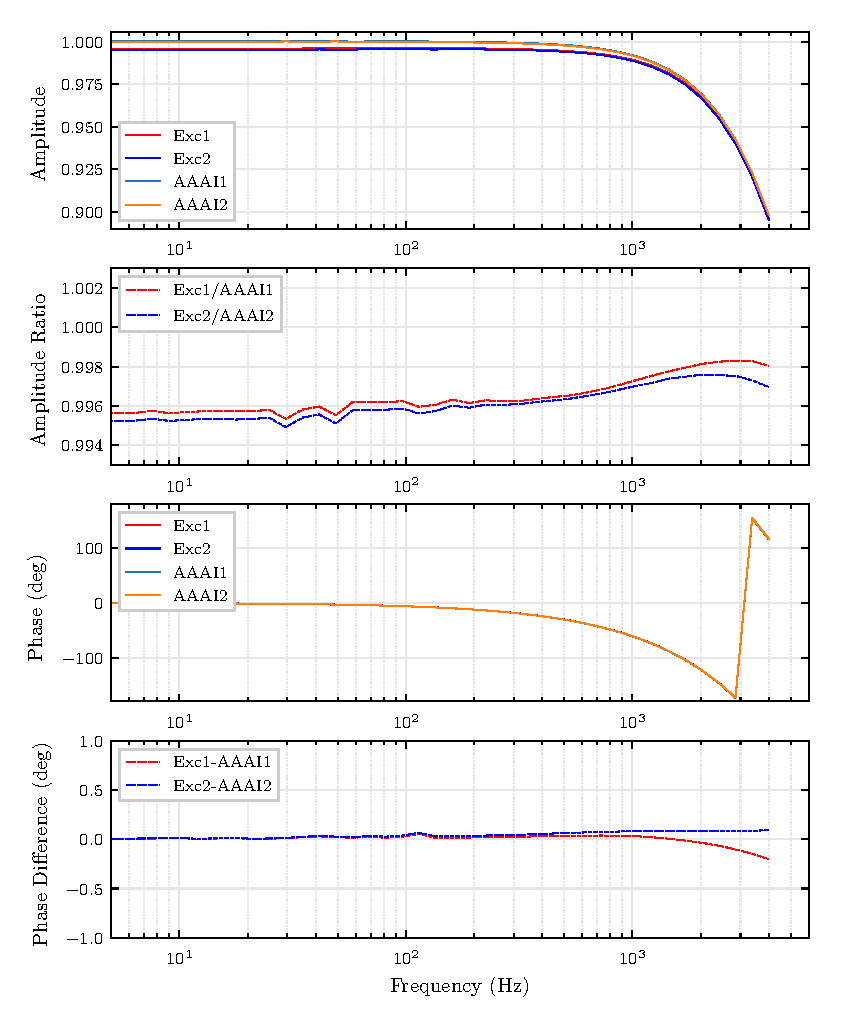
\includegraphics[width=1\textwidth]{figure/tf/TF_KEK_64}
\caption[Transfer function of De-Whitening Filter with Digital Inverse Filter]{Transfer function of De-Whitening Filter with Digital Inverse Filter. The transfer function is measured in KEK cryogenic center with KAGRA standalone digital system and 64kHz salve model.}\label{fig:tf64}
\index{figures}
\end{figure}
%\subsection{Transfer function of Digital Inverse Filter}







\pagebreak
\section{Noise Reduction Performance}
We have tested the noise reduction performance of our De-Whitening Filter in KAGRA X-END. The noise is measured by the KAGRA Digital System with a third order whitening filter, which can amplify the signal above 10Hz for about 60dB. Exactly speaking, it has a third order zero at 10Hz and a third order pole at 1Hz in its amplification circuit. 

The experimental setup is depicted in Fig.~\ref{fig:dew_setup} and Fig.~\ref{fig:dew_setup2m}.\\

\begin{figure}[hbt!]
\centering
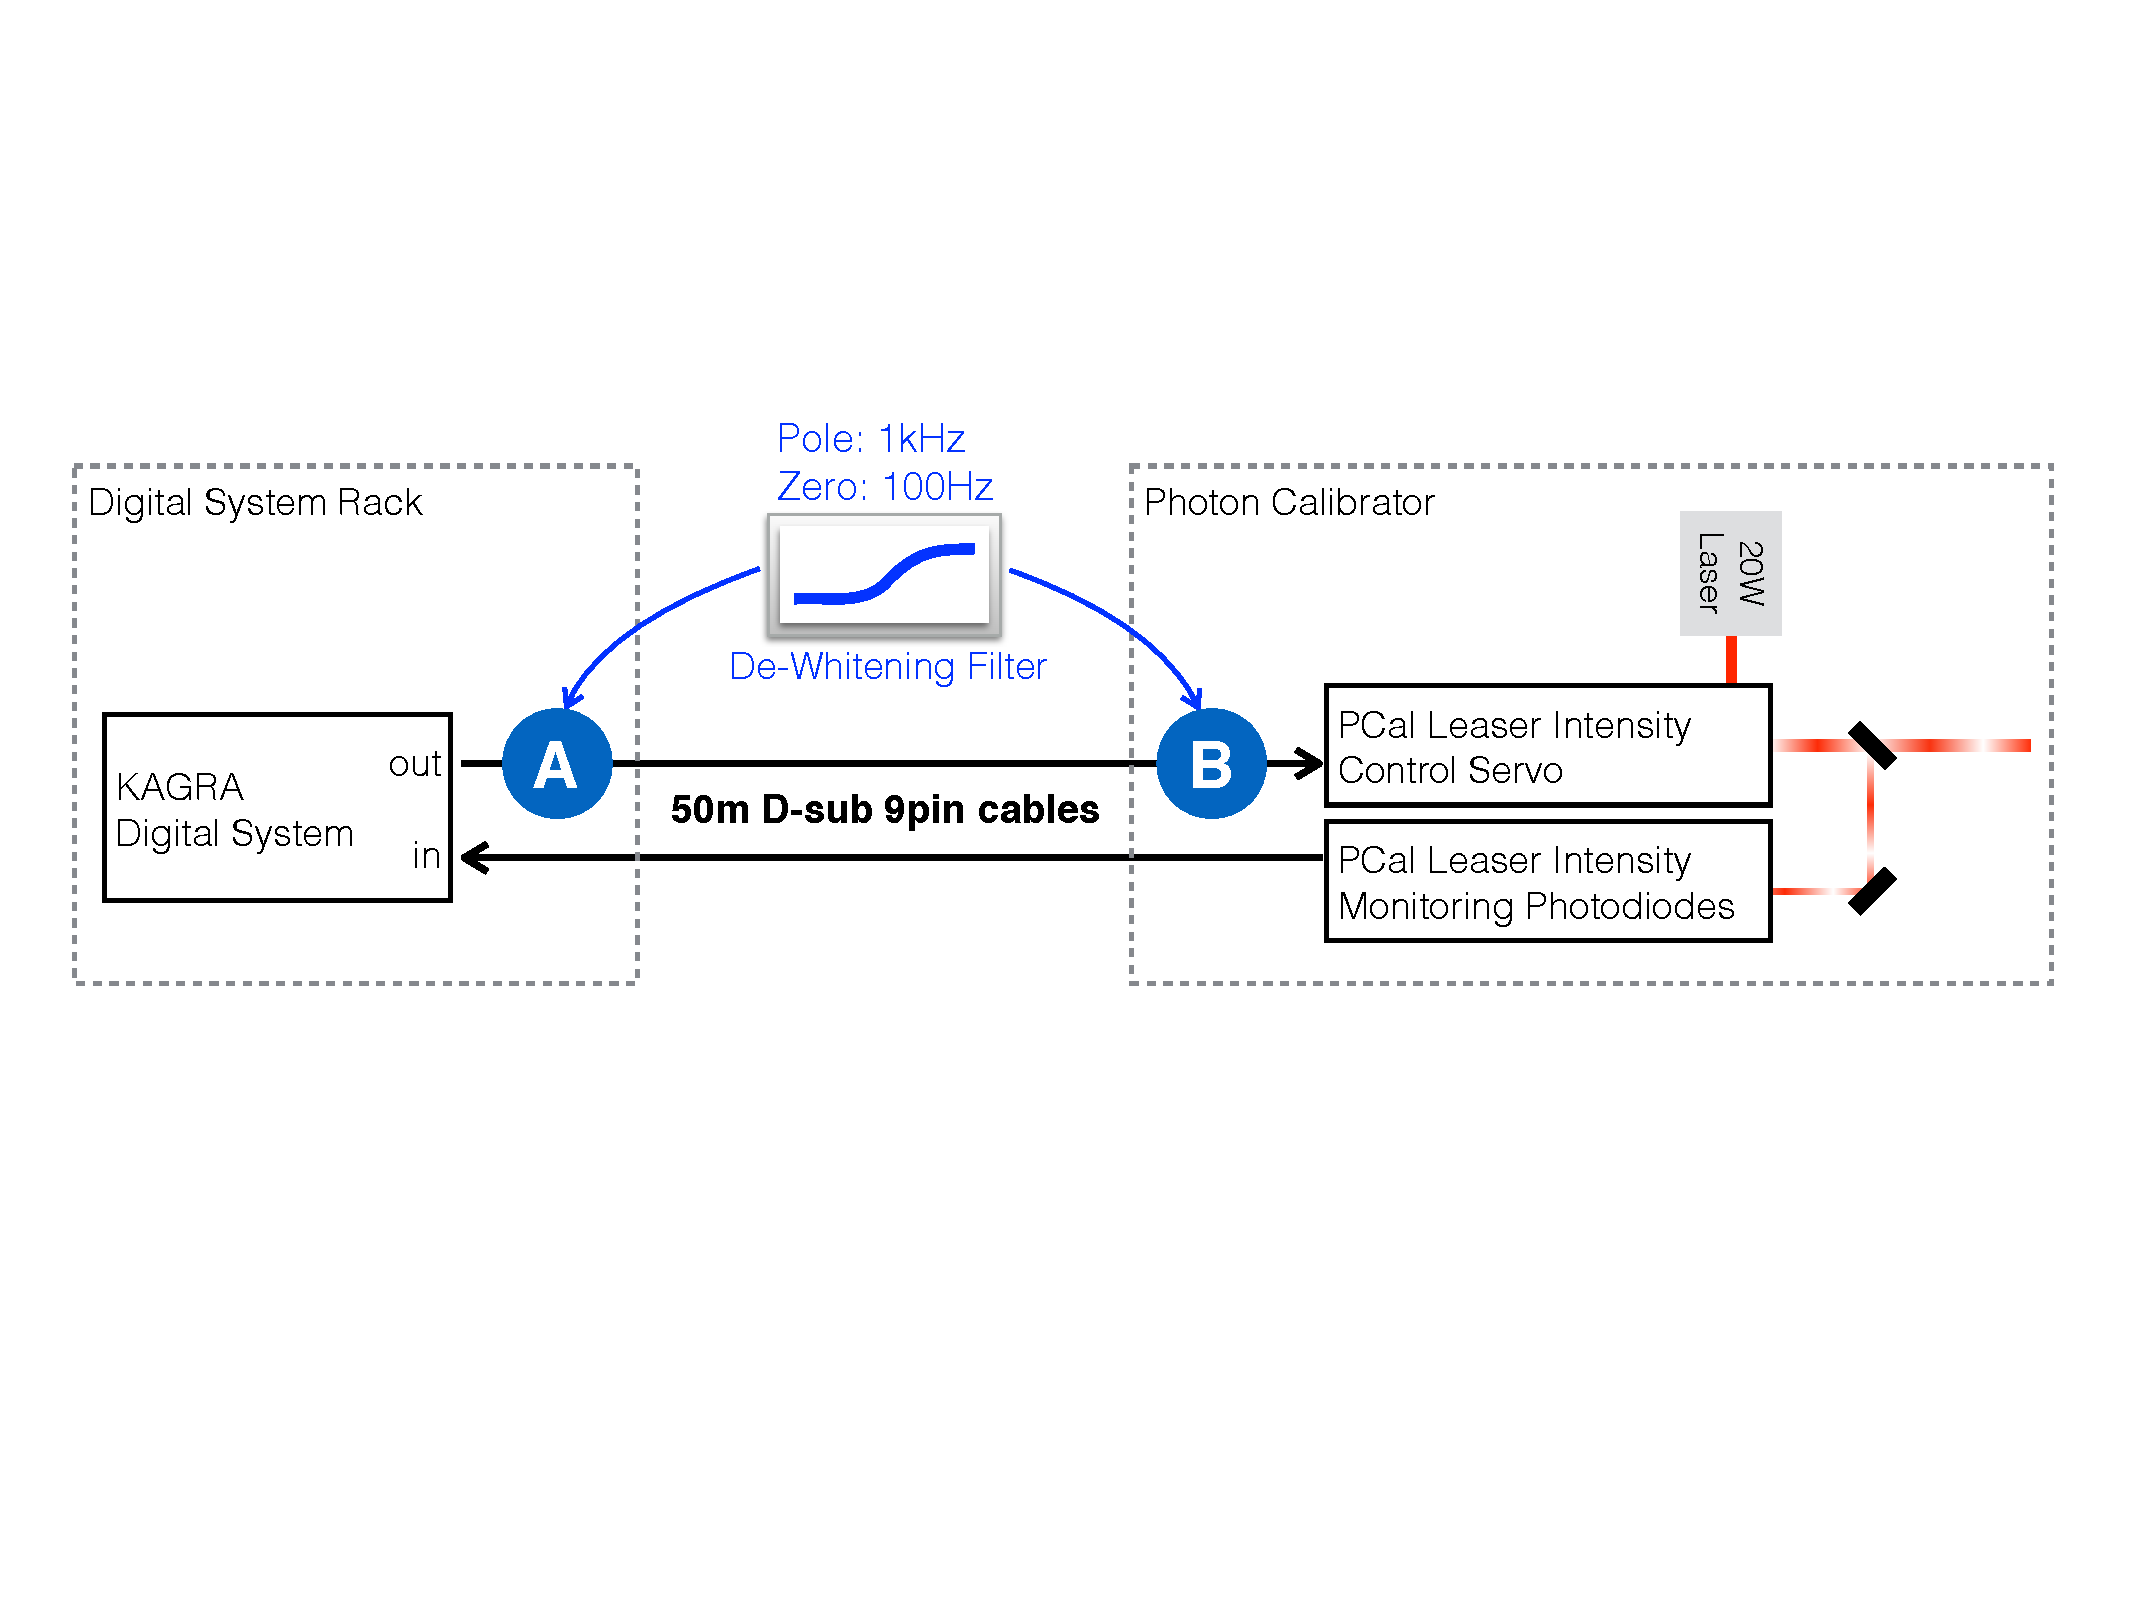
\includegraphics[width=1\textwidth]{figure/dew_setup.pdf}
\caption[Noise Measurement Setup]{In order to reduce the noise coming from the digital system, the De-Whitening filter can be installed at either place A or B.    }
\label{fig:dew_setup}
\index{figures}
\end{figure}

\begin{figure}[hbt!]
\centering
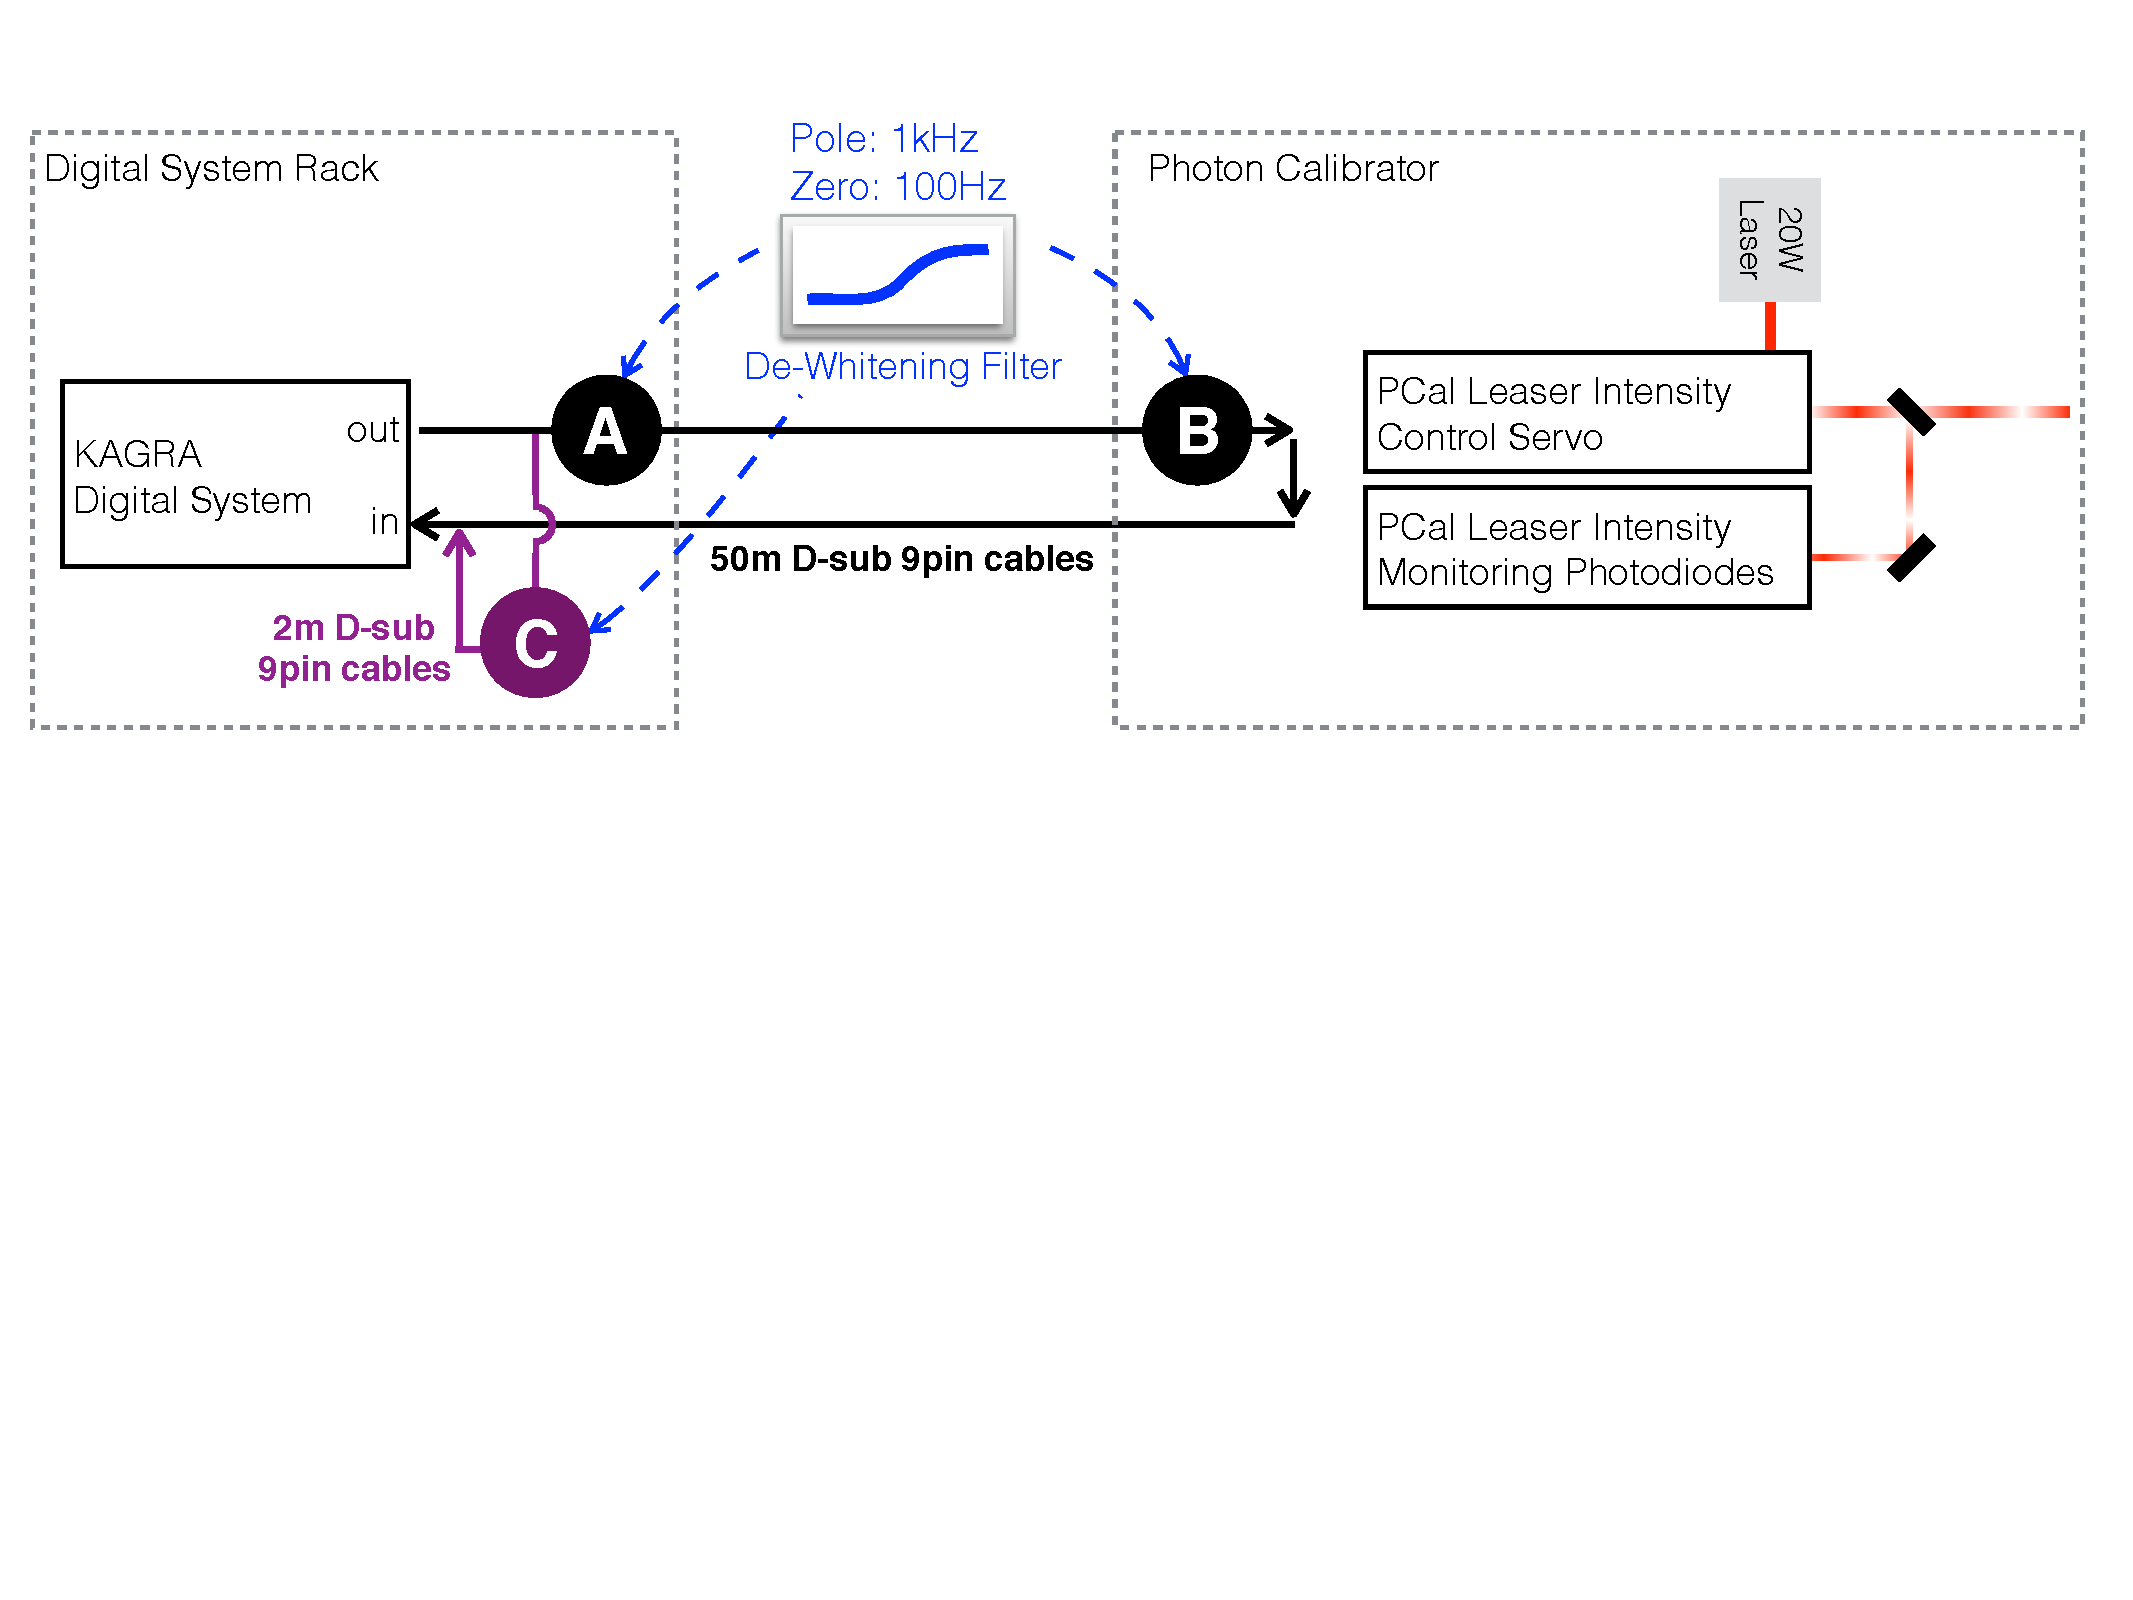
\includegraphics[width=1\textwidth]{figure/dew_setup2m.pdf}
\caption[Noise Measurement Setup]{For our reference, we also measured the noise from the digital system without passing through the control loop of PCal. Place C means we connect De-Whitening filter in digital system rack with 2m cable only in order to investigate the influence from 50m cable.}
\label{fig:dew_setup2m}
\index{figures}
\end{figure}


\pagebreak

The acronym used in legends in measurement plots are explained in Table~\ref{tab:acronym_legend}. \\


\begin{table}[hbt!]
\centering
\begin{tabular}{ll}
\hline
Label in legend  & Description        \\
\hline
AI      & Anti-Alias  Chassis with Whitening Filter (as a preamplifier) \\
AA      & Anti-Image  Chassis   \\
DEW     & De-Whitening Filter   \\
OFS     & Optical-Follower-Servo, the circuit controls PCal laser intensity.\\
\hline
\end{tabular}
\caption{Acronym of devices in noise measurement plots}
\label{tab:acronym_legend}
\index{tables}
\end{table}



\pagebreak
\subsection{Noise Measurement without PCal System}

As described in Fig.(\ref{fig:dew_setup2m}), we have compared the noise from digital control system through different cable length with and without De-Whitening filter.

\begin{figure}[hbt!]
\centering
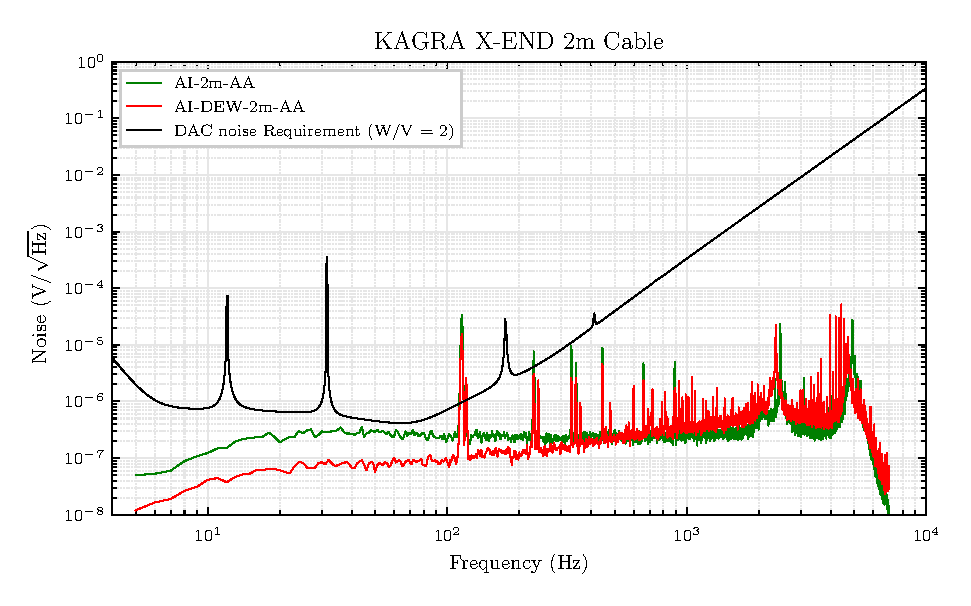
\includegraphics[width=1\textwidth]{figure/noise/00_2m}
\caption[De-Whitening filter noise with short cable]{ De-Whitening filter noise with short (2m) cable. The green line is the noise without De-Whitening filter, while the red one is the noise with De-Whitening filter. Legends indicate relevant devices and cables in their connection order. For example,``AI-DEW-2m-AA" means that the noise measurement includes effects from with an AI filter, a DEW filter, a 2m cable and an AA filter connected in sequence. The list of abbreviations is given in Table~\ref{tab:acronym_legend}  }
\label{fig:00_2m}
\index{figures}
\end{figure}

Fig.(\ref{fig:00_2m}) is the noise measurement result with 2m signal cable as described in Fig.(\ref{fig:dew_setup2m}). The low-frequency noise is suppressed by De-Whitening circuit. However, the amount of suppressing is not 20dB. It is possible that we hit another noise floor at $10^{-7}\mathrm{V}/\sqrt{\mathrm{Hz}}$ due to the internal noise of the De-Whitening filter circuit. Below 10Hz, the measured noise is less than actual noise since we used the a customized high-pass filter, i.e.\ a Whitening Chassis, to prevent the saturation of measurement instrument by any small DC offset. The same effect exists in all noise measurement results in this thesis since we adopted same measuring scheme.


In the end station of KAGRA, unfortunately, the digital system rack is placed near the ETM, which is 36m far away from PCal system. Therefore, the practical control signal is carried by 50m D-sub cables as illustrated in Fig.(\ref{fig:dew_setup}) at this moment. As a result, we tried to perform the same noise measurement with 50m cables. The result is in Fig.(\ref{fig:00_50m}).
\begin{figure}[hbt!]
\centering
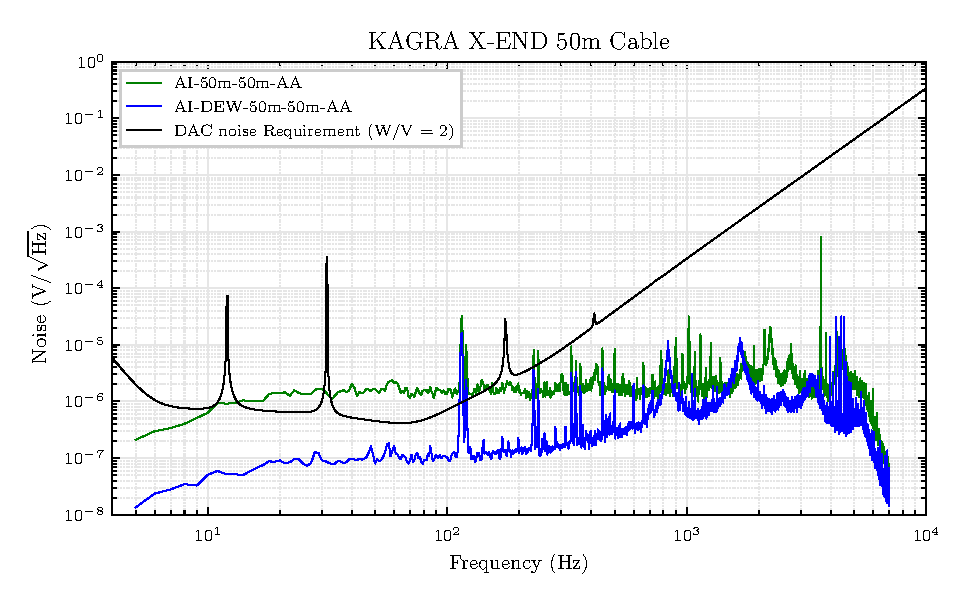
\includegraphics[width=1\textwidth]{figure/noise/00_50m}
\caption[De-Whitening filter noise with long cable]{ De-Whitening filter noise with long (50m) cable. }
\label{fig:00_50m}
\index{figures}
\end{figure}

With 50m cable, the unsuppressed noise (green line in Fig.(\ref{fig:00_50m})) is larger than the one with 2m cable (green line in Fig.(\ref{fig:00_2m})) due to unknown reason. However, the 20dB suppression capability below 100 Hz can be verified in Fig.(\ref{fig:00_50m}). 





\begin{figure}[hbt!]
\centering
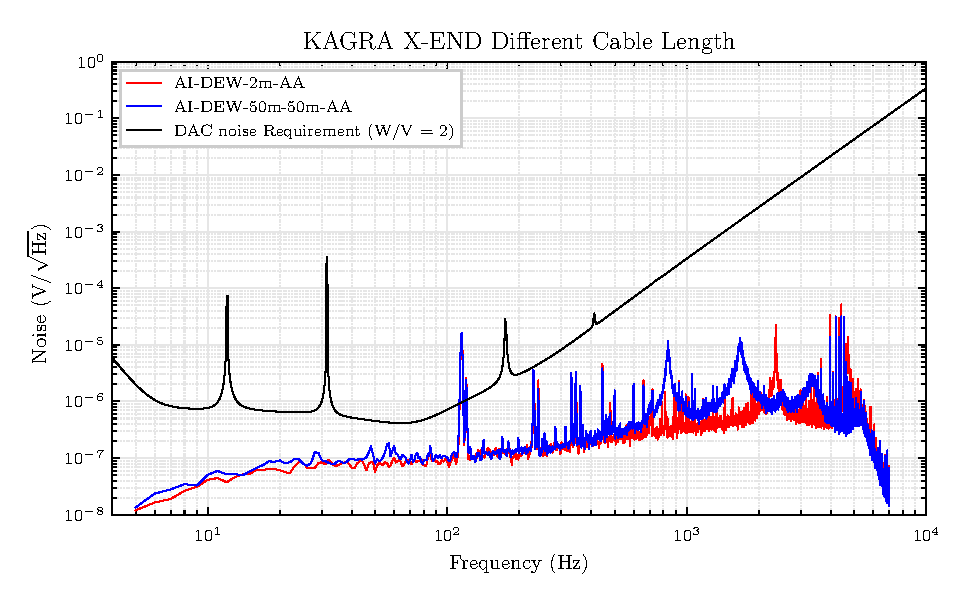
\includegraphics[width=1\textwidth]{figure/noise/00_bothm}
\caption[De-Whitening filter noise with different cable length]{ De-Whitening filter noise with different cable length. }
\label{fig:00_bothm}
\index{figures}
\end{figure}



In Fig.(\ref{fig:00_bothm}), we overplot the suppressed noise by De-Whitening filter in 2m and 50m cable case. Although the 50m case has some noise excess around kHz regime, their low-frequency noise performance do not have significant difference. This result imply that the $10^{-7}\mathrm{V}/\sqrt{\mathrm{Hz}}$ noise floor can really come from De-Whitening circuit itself. In the future, we may come back into this issue when we have more strict noise requirement that will be the case if we decide to use higher power Pcal laser or have better interferometer sensitivity.

Since we observed that the unattenuated noise floor in 50m cable case is larger, we suspect that some environmental noises are picked up by the cable. We tried to install our De-Whitening filter in either place A or B in Fig.\ref{fig:dew_setup2m} and the noise measurement results are shown in Fig.\ref{fig:00_DSP}. Originally, we thought if the extra noise is picked up by the cable, it should be attenuated when we install the De-Whitening filter at place B. However, the red line in Fig.\ref{fig:00_DSP} shows that if we put our De-Whitening filter at place B, the measured noise is actually higher than the one without De-Whitening filter. 


\begin{figure}[hbt!]
\centering
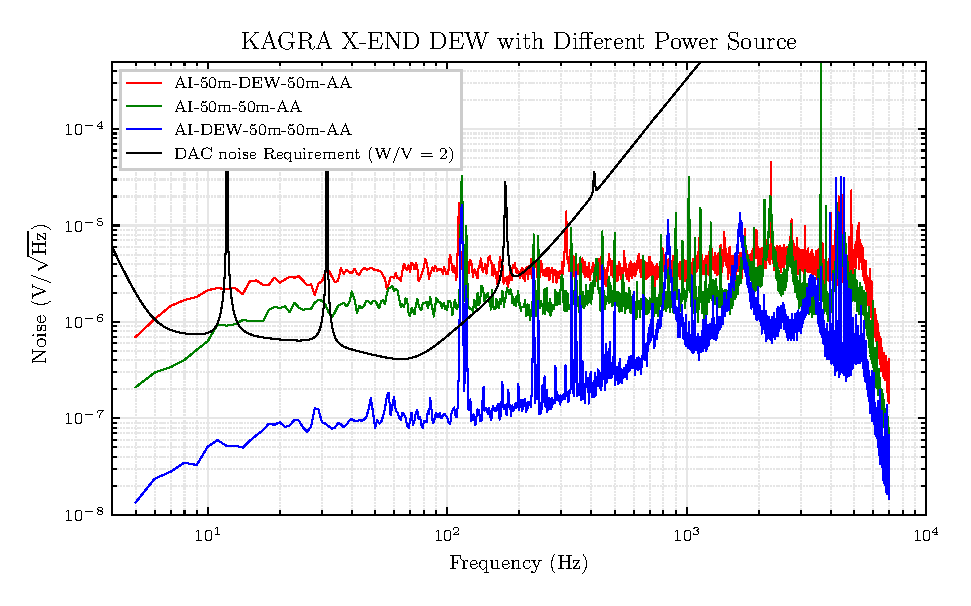
\includegraphics[width=1\textwidth]{figure/noise/00_DSP}
\caption[Noise measurement when the De-Whitening filter is installed at different location]{ Noise measurement when the De-Whitening filter is installed at different location. }
\label{fig:00_DSP}
\index{figures}
\end{figure}

\clearpage

\subsection{Noise Measurement with PCal System}
Now, it is the time to connect the Digital System and the De-Whitening filter to our Photon Calibrator. The practical setup is illustrated in Fig.~\ref{fig:dew_setup}.

First, we try to understand how much low-frequency noise could be suppressed by De-Whitening filter. However, Fig.~\ref{fig:01_all} indicates that something bad happened. Even though in the case with the De-Whitening, the noise decreases from blue line to red line in Fig.~\ref{fig:01_all}, it dose not follow the transfer function of De-Whitening filter, which can only suppress low-frequency noise.

\begin{figure}[hbt!]
\centering
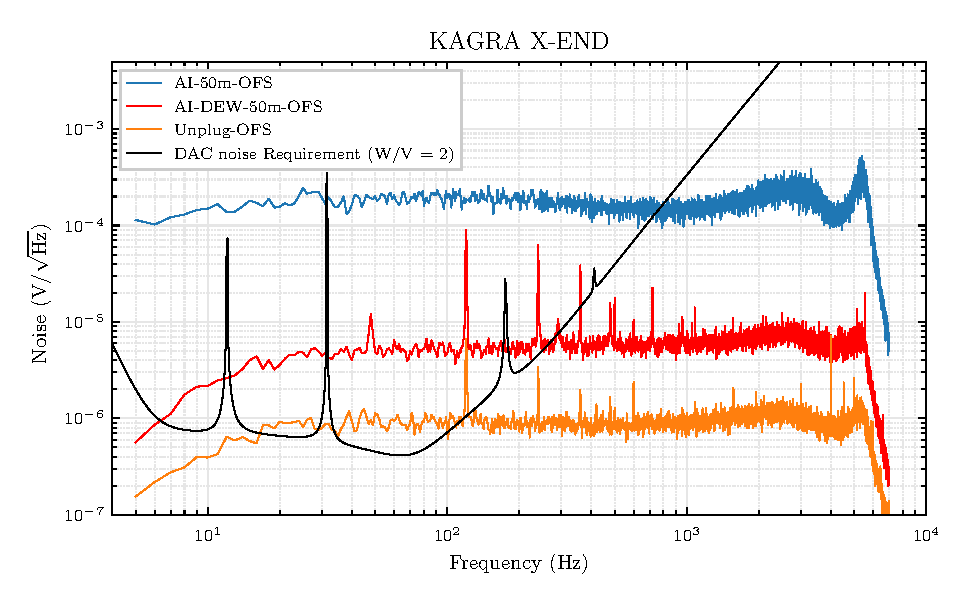
\includegraphics[width=1\textwidth]{figure/noise/01_all}
\caption[Noise measurement with PCal]{ Noise measurement with PCal. These noises can be considered as laser intensity noises since we are measuring photodiode readout as depicted in Fig.~\ref{fig:dew_setup}. The blue line is the case without De-Whitening filer, while the red line is the case when De-Whitening filer has been installed at place A in Fig.~\ref{fig:dew_setup}. The orange line is measured when we disconnect our signal cable from the Laser Intensity Control Servo input port.}
\label{fig:01_all}
\index{figures}
\end{figure}

On the other hand, the orange line is the nosies when we disconnect the digital system output from our PCal. It is lower than either one of connected cases (blue and red). Besides, it is also higher than the noise that are plotted in Fig.(\ref{fig:00_bothm}), which is supposed to be the noise sent to PCal from the output of De-Whitening filter. It reveals that the blue and the red lines in Fig.~\ref{fig:01_all} are actually popped out just when we connect the digital system and our PCal together. We doubt that we may create the infamous grounding loop unintentionally. As a trial, we did two different measurements. First, we put our De-Whitening filter in either palace A or B in Fig.~\ref{fig:dew_setup} and the result is in Fig.~\ref{fig:01_AvsB}. Second, we supplied our Pcal from the DC power source located at digital system rack, which is shared with De-Whitening filter and other analog chassis of the digital system, including Anti-Image, Anti-Alias, and Whiting chassis. The result is given in Fig.~\ref{fig:01_SP}.

\begin{figure}[hbt!]
\centering
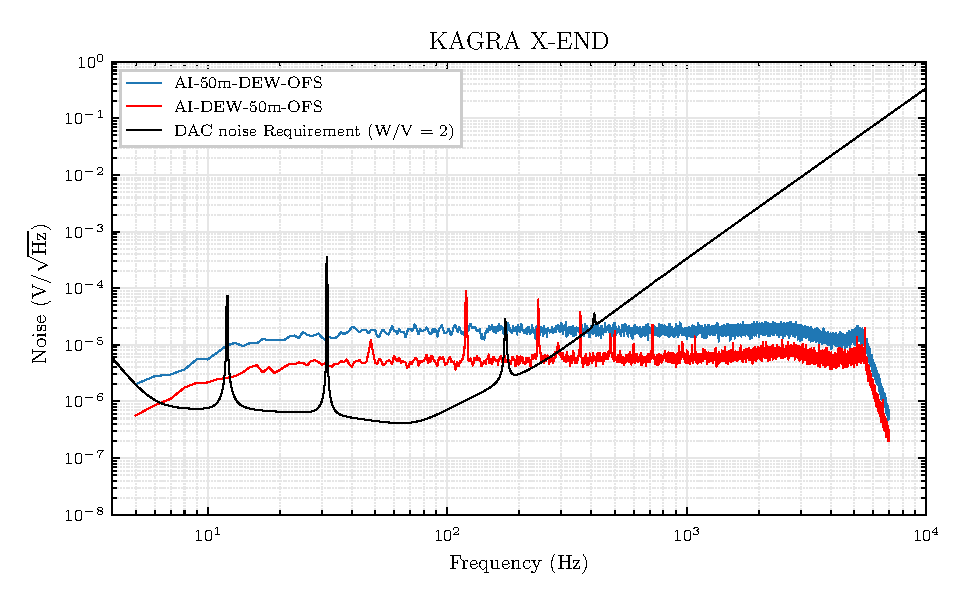
\includegraphics[width=1\textwidth]{figure/noise/01_AvsB}
\caption[Noise measurement with PCal and different location of the De-whitening]{ The red line and the blue line are measured when De-whitening is located at Place A and Place B in Fig.~\ref{fig:dew_setup} respectively.}
\label{fig:01_AvsB}
\index{figures}
\end{figure}

Fig.~\ref{fig:01_AvsB} shows that if we install our De-Whitening filter at Place B in Fig.~\ref{fig:dew_setup}, we got a higher noise floor. The similar effect has been observed in Fig.~\ref{fig:00_DSP}. 

\pagebreak

\begin{figure}[hbt!]
\centering
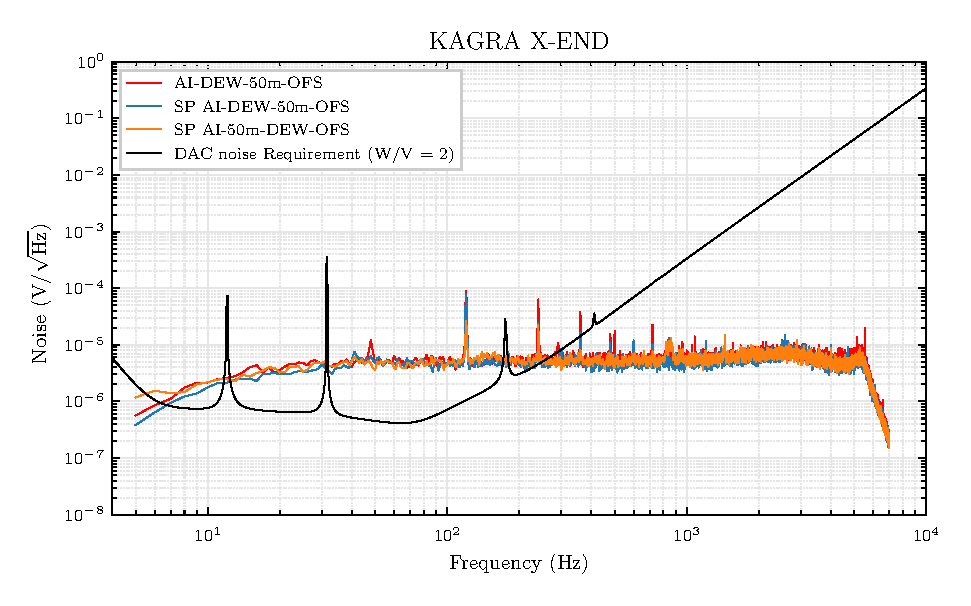
\includegraphics[width=1\textwidth]{figure/noise/01_SP}
\caption[Noise measurement with PCal and different power source]{ Lines labeled with ``SP'' were measured when we supplied digital system, De-Whitening filter and PCal with Same Power source located in digital system rack. }
\label{fig:01_SP}
\index{figures}
\end{figure}

When we supply our PCal with the shared power source in the digital system rack, the noise floors become independent of the location of the De-Whitening filter as you can observe in Fig.~\ref{fig:01_SP}. They are also coincident with the red line in the plot. Among measurements we have tried, whenever the De-Whitening filter is supplied by the same power source as the Anti-Image chassis, which is the upstream device of De-Whitening filter, the noise floor became the same as the red line in Fig.~\ref{fig:01_SP}.
